\documentclass [aspectratio=169]{beamer}
\beamertemplatenavigationsymbolsempty
\usetheme{Boadilla}
\usepackage{textpos} % package for the positioning
\usepackage[]{graphicx}
\usepackage{graphicx}
\usepackage{float}
\usepackage{hyperref}
\usepackage{caption}
\usepackage{subcaption}
\usepackage{algorithm,algpseudocode}
\usepackage[export]{adjustbox}
\usepackage{tikz}
\usepackage[square,numbers]{natbib}
\usepackage[byname]{smartref}
\usetikzlibrary{positioning}
\usetikzlibrary{arrows, shapes, decorations, automata, backgrounds, fit, petri, calc}

\newcommand*{\logofont}{\fontfamily{phv}\selectfont}

\definecolor{uwopurple}{RGB}{1,38,131} % official purple color for uwo

\title[]{\vspace{60pt} \\
Seleção de meta-features e seu efeito na performance de sistemas de meta-aprendizagem} 

\author[]{João Pedro Nunes Magalhães \and Victor Hugo Silva Ângelo}
\institute[]{\textbf{Instituto de Computação (IC)}\\
\textbf{Universidade Federal de Alagoas (UFAL)}}
\date{\today}

% Math notations
\newtheorem{thm}{Theorem}[section]
\newtheorem{lem}[thm]{Lemma}
\newtheorem{defn}[thm]{Definition}
\newtheorem{eg}[thm]{Example}
\newtheorem{ex}[thm]{Exercise}
\newtheorem{conj}[thm]{Conjecture}
\newtheorem{cor}[thm]{Corollary}
\newtheorem{claim}[thm]{Claim}
\newtheorem{rmk}[thm]{Remark}

\newcommand{\ie}{\emph{i.e.} }
\newcommand{\cf}{\emph{cf.} }
\newcommand{\into}{\hookrightarrow}
\newcommand{\dirac}{\slashed{\partial}}
\newcommand{\R}{\mathbb{R}}
\newcommand{\C}{\mathbb{C}}
\newcommand{\Z}{\mathbb{Z}}
\newcommand{\N}{\mathbb{N}}
\newcommand{\Q}{\mathbb{Q}}
\newcommand{\LieT}{\mathfrak{t}}
\newcommand{\T}{\mathbb{T}}
\newcommand{\A}{\mathds{A}}
\newcommand{\E}{\mathbb{E}}
\newcommand{\Prob}{\mathbb{P}}
\newcommand{\Var}{\text{Var}}
\newcommand\equalhat{%
\let\savearraystretch\arraystretch
\renewcommand\arraystretch{0.3}
\begin{array}{c}
\stretchto{
    \scalerel*[\widthof{=}]{\wedge}
    {\rule{1ex}{3ex}}%
}{0.5ex}\\ 
=%
\end{array}
\let\arraystretch\savearraystretch
}

% set color
\setbeamercolor{title in head/foot}{bg=white}
\setbeamercolor{author in head/foot}{bg=white}
\setbeamercolor{date in head/foot}{fg=uwopurple}
\setbeamercolor{date in head/foot}{bg=white}
\setbeamercolor{title}{fg=uwopurple}
\setbeamerfont{title}{series=\bfseries}
\setbeamercolor{frametitle}{fg=uwopurple}
\setbeamerfont{frametitle}{series=\bfseries}
\setbeamercolor{item}{fg=uwopurple}
\setbeamercolor{caption name}{fg=uwopurple!70!}

% set logo at non-title pages
\logo{
\includegraphics[height=0.9cm]{logo.png}\vspace*{-.055\paperheight}\hspace*{.85\paperwidth}}

\begin{document}

{
\setbeamertemplate{logo}{}
\begin{frame}
    \titlepage
    \begin{textblock*}{4cm}(5.5cm,-8.3cm)
        
\includegraphics[width=4cm]{logo.png}
    \end{textblock*}
\end{frame}
}

\begin{frame}{Sumário}
    \begin{block}{}
        \begin{enumerate}
            \item Introdução e Motivação
            \item O Problema
            \item Proposta (Exatos, Aproximados, Híbrido)
            \item Metodologia Experimental
            \item Resultados
            \item Conclusão
        \end{enumerate}
    \end{block}
\end{frame}

\section{Introdução e Motivação}

\begin{frame}{Introdução e Motivação}
\begin{block}{Contexto AutoML}
A importância de selecionar os atributos corretos para a construção de metamodelos é fundamental para otimizar recomendações de algoritmos \cite{vanschoren2018meta, he2021automl, wang2023onestep}.
\end{block}

\vspace{0.3cm}

\begin{itemize}
    \item \textbf{Alta dimensionalidade:} Bibliotecas geram milhares de descritores (meta-features).
    \item \textbf{Impacto negativo:} Comprometimento do treinamento, aumento de ruído, e elevado consumo computacional.
    \item \textbf{Desafio prático:} Reduzir as meta-features de forma eficiente para maximizar acertos do classificador no nível meta.
\end{itemize}
\end{frame}

\section{O Problema}

\begin{frame}{O Problema}
\begin{block}{Otimização Combinatória}
O problema central consiste na busca de um subconjunto de características que maximize a acurácia preditiva.
\end{block}

\vspace{0.3cm}
\begin{itemize}
    \item Avaliar todas as combinações discretas de atributos é \textbf{intratável} do ponto de vista computacional.
    \item Precisamos aplicar abordagens de \textbf{Pesquisa Operacional} e \textbf{Meta-Heurísticas} para filtrar as informações mais relevantes.
\end{itemize}
\end{frame}

\section{Proposta}

\begin{frame}{Proposta}

\begin{block}{Seleção do melhor subconjunto de meta-features}
Identificar um subconjunto de meta-features capaz de elevar a acurácia do meta-modelo sob a estratégia de recomendação do melhor algoritmo (\textit{Best Algorithm}).\end{block}

\begin{itemize}
    \item \textbf{Caracteristicas do meta-dataset:} Utilizar o meta-dataset com meta-features de 94 datasets do \textit{openml} (Exemplo 4), tendo 1153 meta-features extraídas.
    \item \textbf{Maximizar acuracia:} Encontrar um subconjunto que maximiza a acuracia do meta-modelo.
    \item \textbf{Meta-features com pré processamento vs sem pré processamento:} Metodo exato não utiliza pré processamento para melhorar o desempenho, porém os métodos aproximados e abordagem hibrida utilizam pré processamento para melhorar o desempenho.
\end{itemize}
\end{frame}

\begin{frame}{Proposta - Métodos Exatos}
Adaptação de modelagens matemáticas consolidadas na Literatura, extraindo coeficientes de importância dos modelos (\textit{Feature Importances}).

\begin{itemize}
    \item \textbf{Melhor Subconjunto:} Restrição de igualdade estrita para a cardinalidade.
    \item \textbf{Mochila com Penalidades:} Teto flexível de capacidade e aplicação de penalidade para atributos de baixo ganho.
    \item \textbf{Mochila Quadrática Linearizada:} Foca em penalizar a seleção de variáveis redundantes baseando-se no índice de \textbf{correlação} entre elas, utilizando inequações de McCormick.
\end{itemize}
\end{frame}

\begin{frame}{Proposta - Métodos Aproximados}
Utilização de Algoritmos Genéticos (AG) para contornar a intratabilidade. Soluções são representadas vetorialmente de forma binária.

\begin{itemize}
    \item \textbf{AG Clássico:} Exploração estocástica pura, funcionando como linha de base.
    \item \textbf{AG Guiado (MI + Busca Local):} A população inicial sofre injeção de qualidade baseada na relevância \textit{Mutual Information}.
    \item \textbf{AG Esparso:} Focado em obter subconjuntos compactos, controlando ativamente a proporção máxima de genes selecionados.
\end{itemize}
\end{frame}

\begin{frame}{Proposta - Abordagem Híbrida}
\begin{block}{Seeded GA}
A Abordagem Híbrida utiliza os resultados provenientes dos Modelos Exatos (Programação Linear Inteira) como pré-processamento.
\end{block}

\vspace{0.3cm}
\begin{itemize}
    \item Em contraste a abordagens focadas puramente na qualidade basal \cite{nayak2022ontological}, os melhores arranjos encontrados pelos métodos matemáticos exatos são inseridos como indivíduos \textbf{Elite} na população inicial do AG.
    \item Une a exatidão e rigor da Pesquisa Operacional com a capacidade extrema de exploração topográfica dos Algoritmos Genéticos.
\end{itemize}
\end{frame}

\section{Metodologia Experimental}

\begin{frame}{Metodologia Experimental - Métodos Exatos}
\begin{block}{Execução e Extração}
\begin{itemize}
    \item \textbf{Pré-Processamento:} Sem aplicação de transformação ou seleção de dados prévia na base.
    \item \textbf{Classificadores Base Nível Meta:} Avaliados utilizando Decision Tree, Random Forest, SVM, KNN e Naive Bayes.
    \item \textbf{Validação Cruzada:} O sistema baseou-se inteiramente na técnica rigorosa de \textit{Leave-One-Out} (LOOCV).
\end{itemize}
\end{block}
\end{frame}

\begin{frame}{Metodologia Experimental - Métodos Aproximados}
\begin{block}{Pré-Processamento e Purificação}
\begin{itemize}
    \item \textbf{Limpeza:} Redução drástica nas meta-features brutas por filtros estáticos (baixa variância, colinearidade, NaNs).
    \item \textbf{Filtro:} Utilização de \textit{Mutual Information} culminando num grupo refinado de 150 top características.
\end{itemize}
\end{block}

\vspace{0.3cm}
\begin{block}{Avaliação Iterativa}
\begin{itemize}
    \item \textbf{Motor Genético:} Baseou-se no classificador \textit{ExtraTreesClassifier} (rápido e estável).
    \item \textbf{Validação Cruzada:} Realizada através da técnica de \textit{StratifiedKFold} com $k=5$ agrupamentos.
\end{itemize}
\end{block}
\end{frame}

\begin{frame}{Metodologia Experimental - Abordagem Híbrida}
\begin{block}{União das Estratégias}
A Abordagem Híbrida consolida as etapas metodológicas de ambas as perspectivas anteriores:
\end{block}

\vspace{0.3cm}
\begin{itemize}
    \item Inicialmente, os modelos exatos operam em sua essência (sem pré-processamento de dimensionalidade e sob LOOCV) para resgatar os subconjuntos ótimos.
    \item Em seguida, os Algoritmos Genéticos (\textit{Seeded GA}) adotam essas sementes de elite, rodando sob todo o escopo de pré-processamento (limpeza e filtragem) e efetuando a evolução utilizando validação estratificada (\textit{StratifiedKFold} com $k=5$).
\end{itemize}
\end{frame}

\section{Resultados}

\begin{frame}{Resultados - Métodos Exatos}
\begin{table}[]
\centering
\begin{tabular}{llcc}
\hline
\textbf{Método} & \textbf{Melhor Algoritmo} & \textbf{Acurácia Média} & \textbf{Qtd. Meta-features} \\
\hline
Melhor Subset & Decision Tree & 0.6276 & 200 \\
Knapsack c/ Penalidade & Decision Tree & 0.6808 & 23 \\
Knapsack Quadrática & Decision Tree & 0.6702 & 17 \\
\hline
\end{tabular}
\end{table}

\begin{itemize}
    \item A drástica redução de atributos mantendo a performance corrobora estudos empíricos anteriores \cite{pereira2021evaluating}.
\end{itemize}

\begin{figure}[H]
\centering
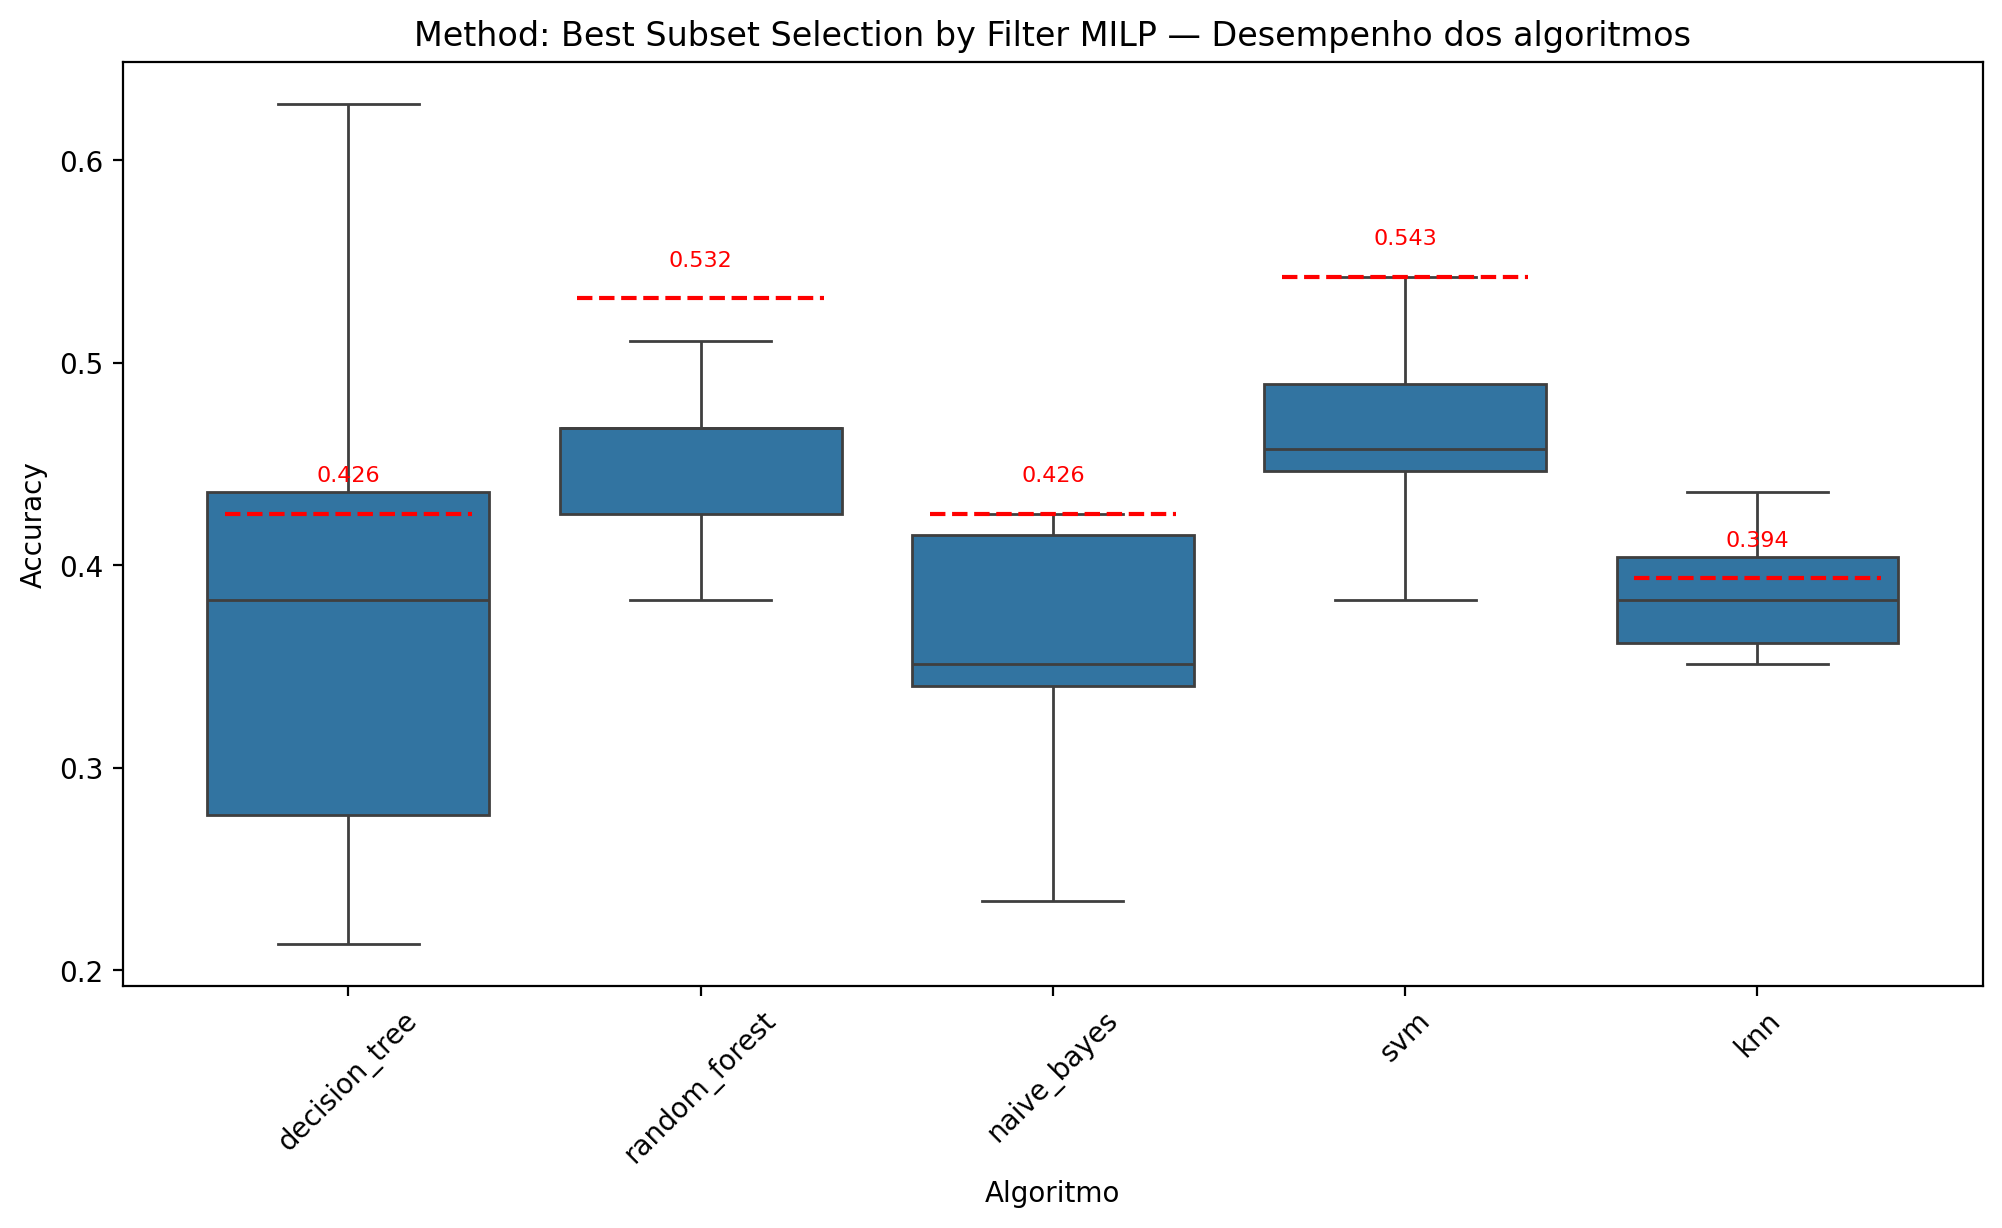
\includegraphics[width=.3\textwidth]{figures/boxplot_method_Best_Subset_Selection_by_Filter_MILP.png}
\hfill
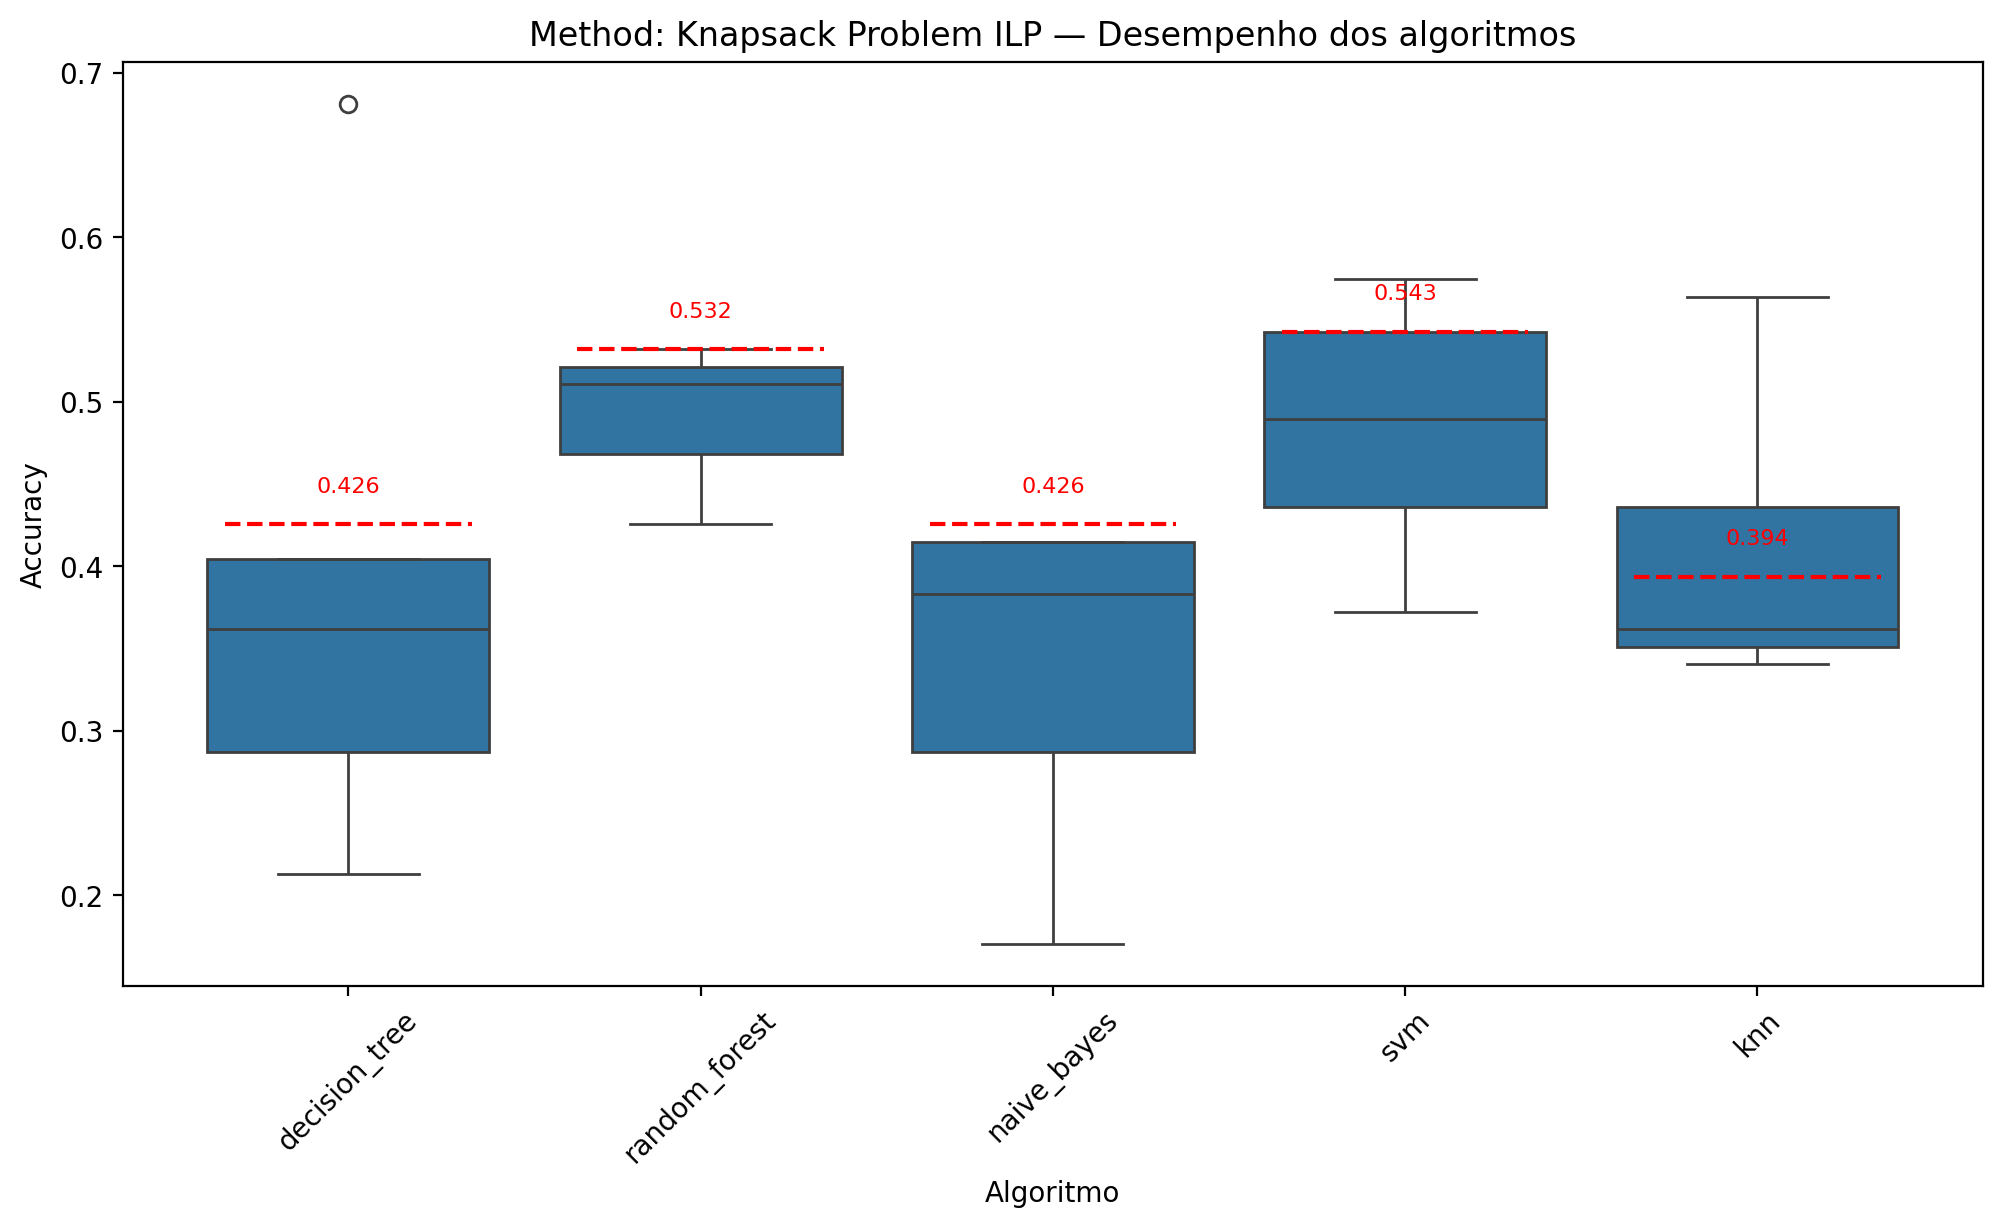
\includegraphics[width=.3\textwidth]{figures/boxplot_method_Knapsack_Problem_ILP.png}
\hfill
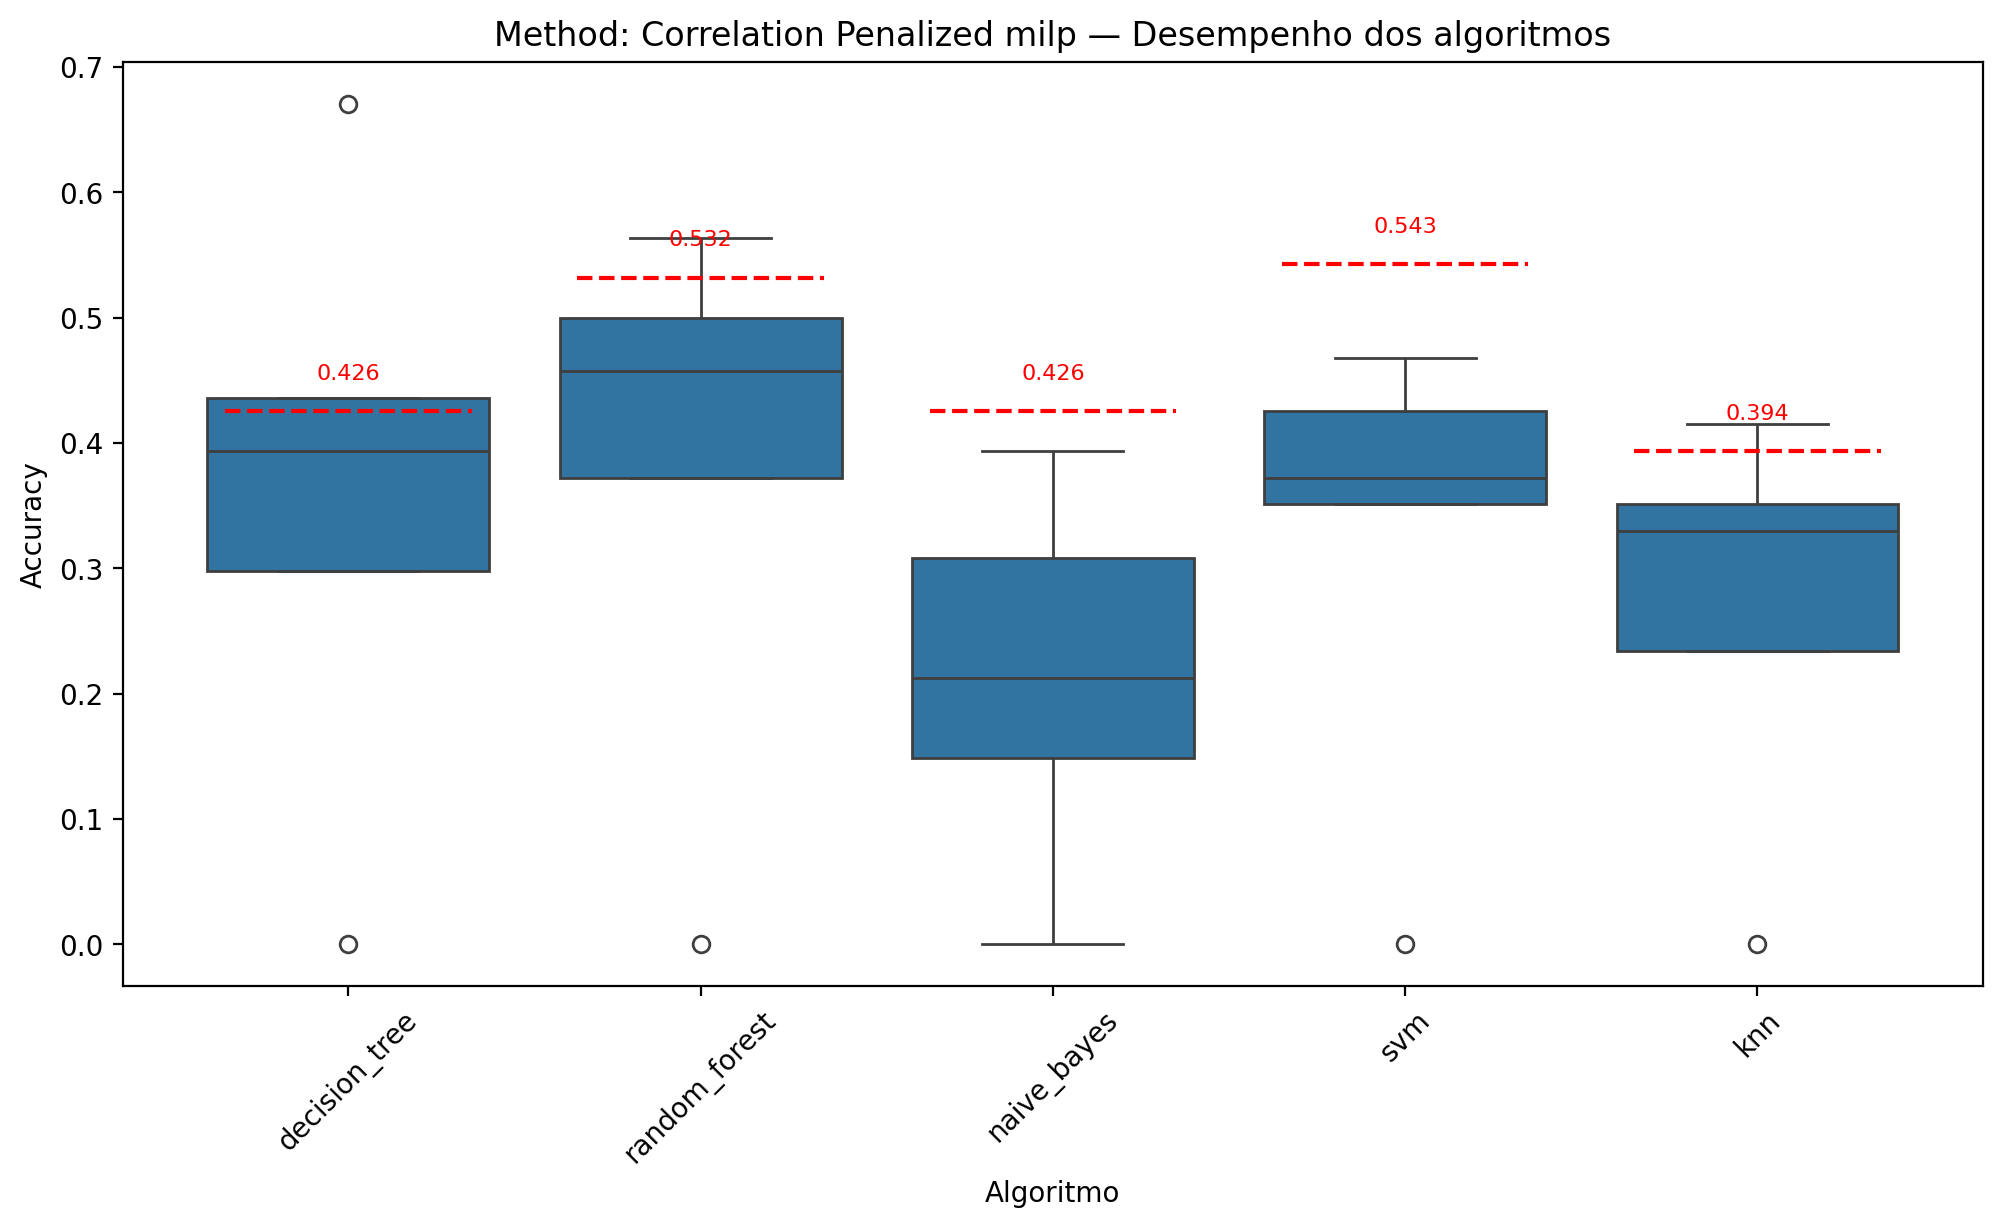
\includegraphics[width=.3\textwidth]{figures/boxplot_method_Correlation_Penalized_milp.png}
\end{figure}
\end{frame}

\begin{frame}{Resultados - Métodos Aproximados}
\begin{table}[]
\centering
\begin{tabular}{lcccc}
\hline
\textbf{Método} & \textbf{Acurácia} & \textbf{Desvio} & \textbf{Qtd. Meta-features} \\
\hline
AG 1 - Clássico & 0,6339 & 0,0542 & 66 \\
AG 2 - Guiado (MI) & 0,6866 & 0,0700 & 31 \\
AG 3 - Esparso & 0,6661 & 0,0723 & 18 \\
\hline
\end{tabular}
\end{table}

\begin{figure}[H]
\centering
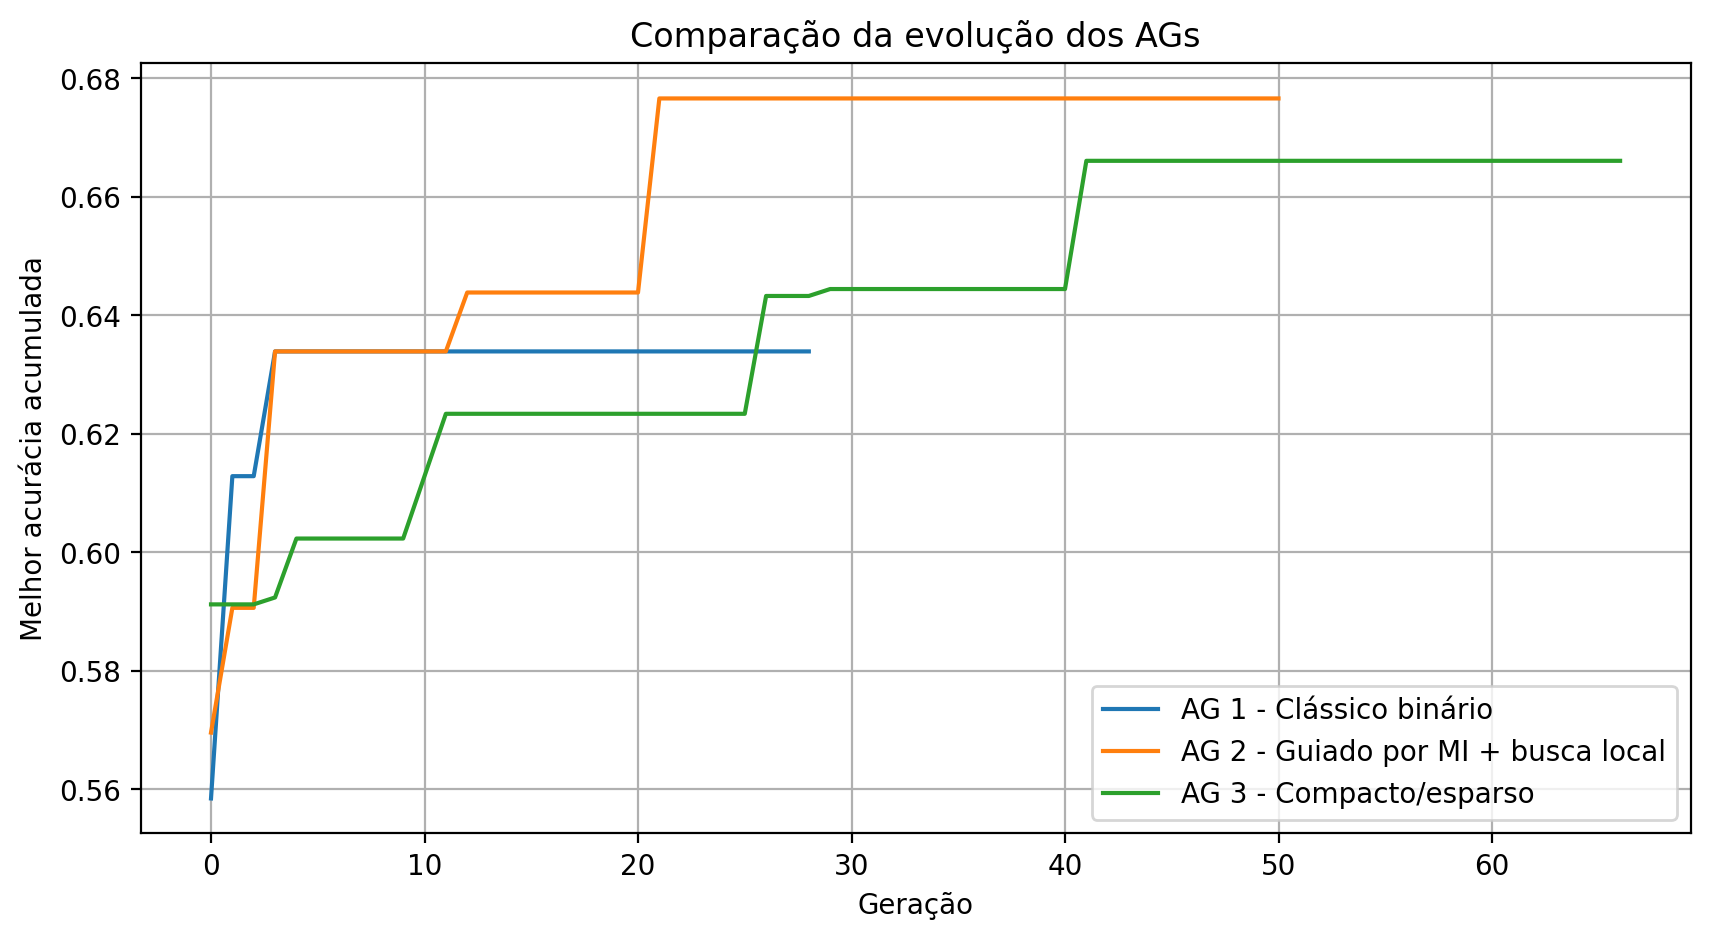
\includegraphics[width=.4\textwidth]{figures/evolution_ag_accuracy.png}
\hfill
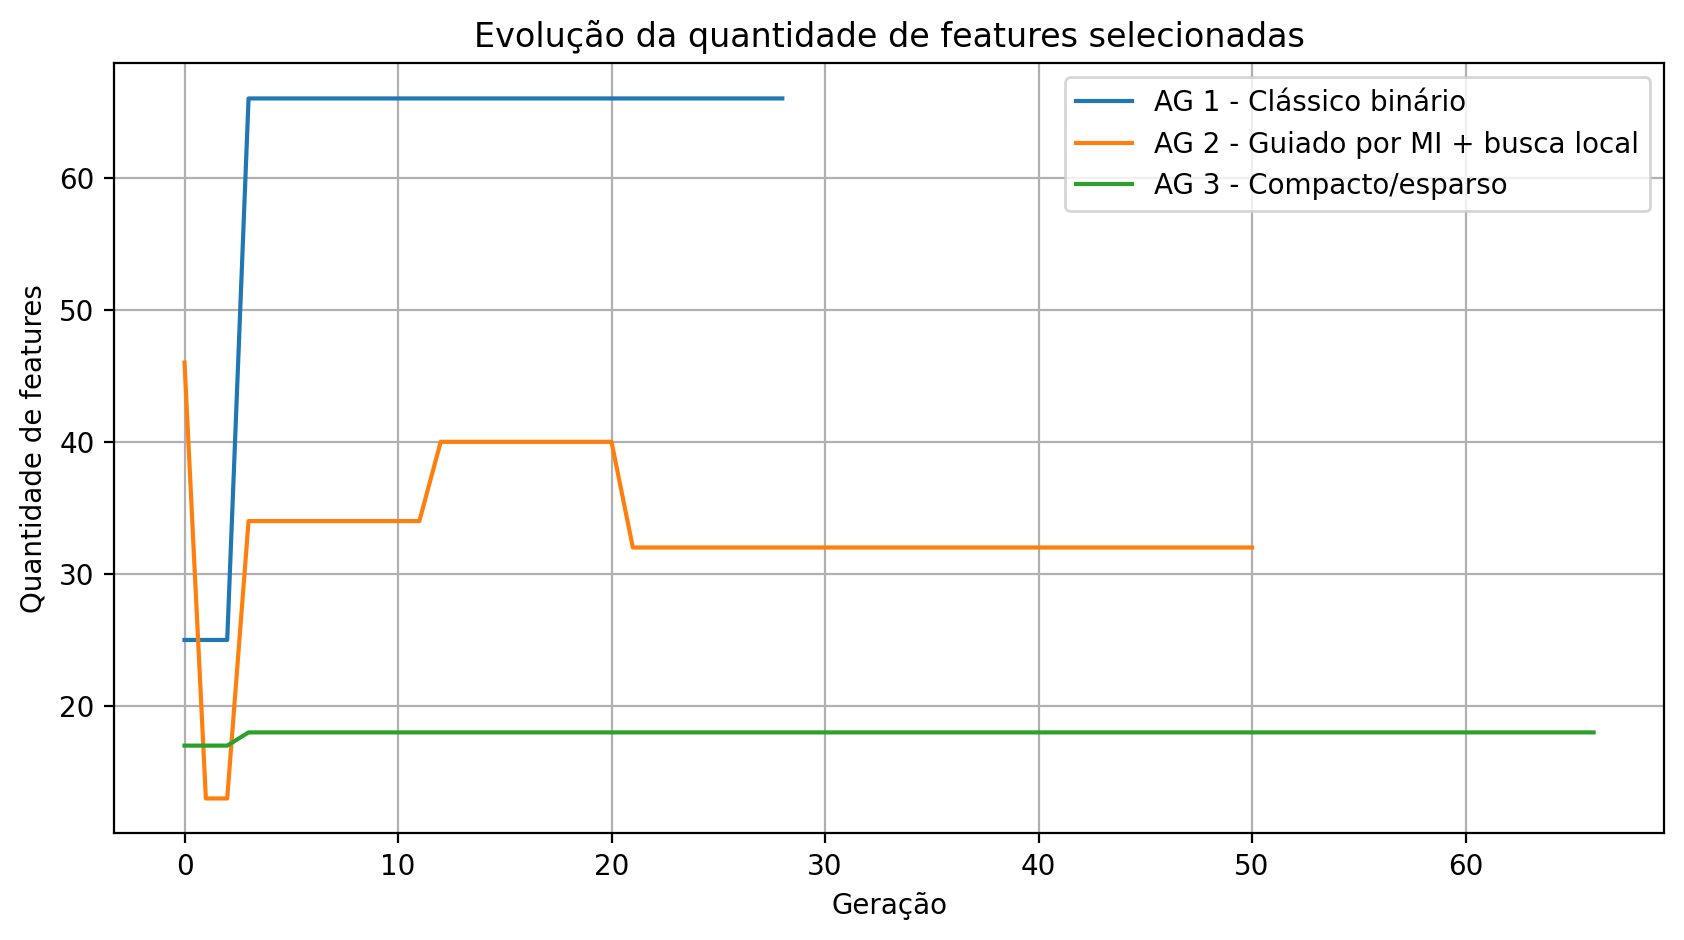
\includegraphics[width=.4\textwidth]{figures/evolution_ag_n_features.png}
\end{figure}
\end{frame}


\begin{frame}{Resultados - Abordagem Híbrida}
\begin{table}[]
\centering
\begin{tabular}{lcccc}
\hline
\textbf{Método} & \textbf{Acurácia} & \textbf{Desvio} & \textbf{Qtd. Meta-features} \\
\hline
Híbrido AG 1 - Clássico & 0,6660 & 0,1037 & 71 \\
Híbrido AG 2 - Guiado & 0,6649 & 0,1084 & 30 \\
Híbrido AG 3 - Esparso & 0,7105 & 0,0954 & 18 \\
\hline
\end{tabular}
\end{table}

\begin{itemize}
    \item A Abordagem Híbrida (AG Esparso) bateu a incrível acurácia de \textbf{71,05\%} necessitando de apenas \textbf{18 atributos}.
\end{itemize}

\begin{figure}[H]
\centering
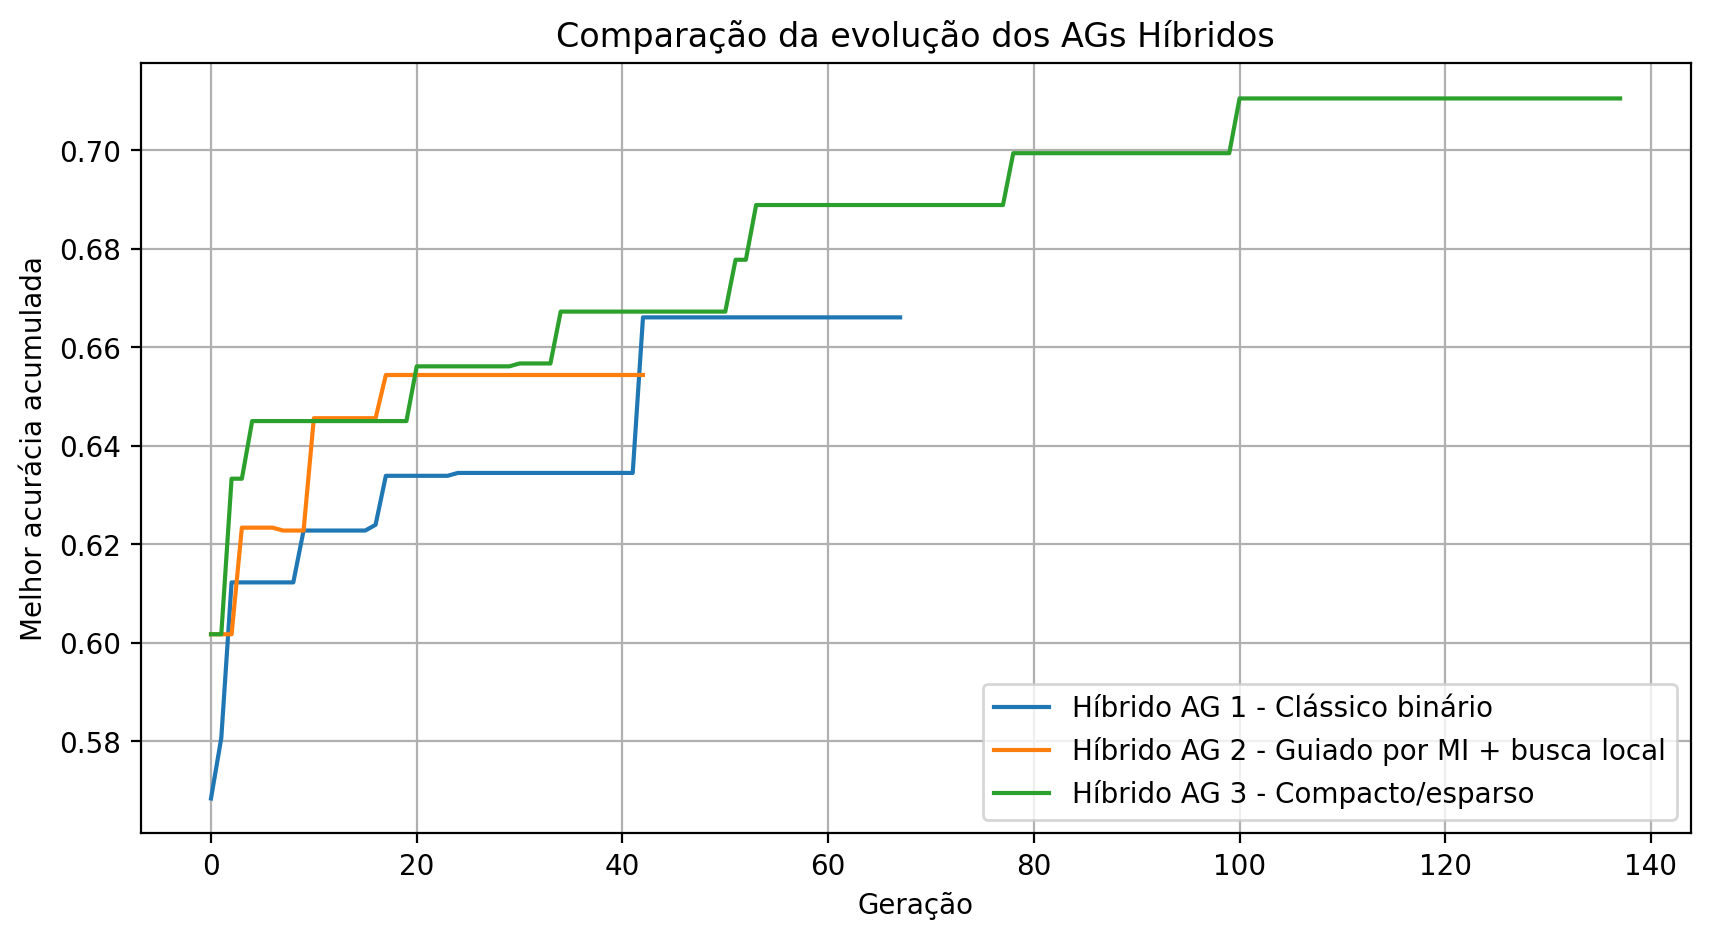
\includegraphics[width=.4\textwidth]{figures/evolution_ag_hybrid_accuracy.png}
\hfill
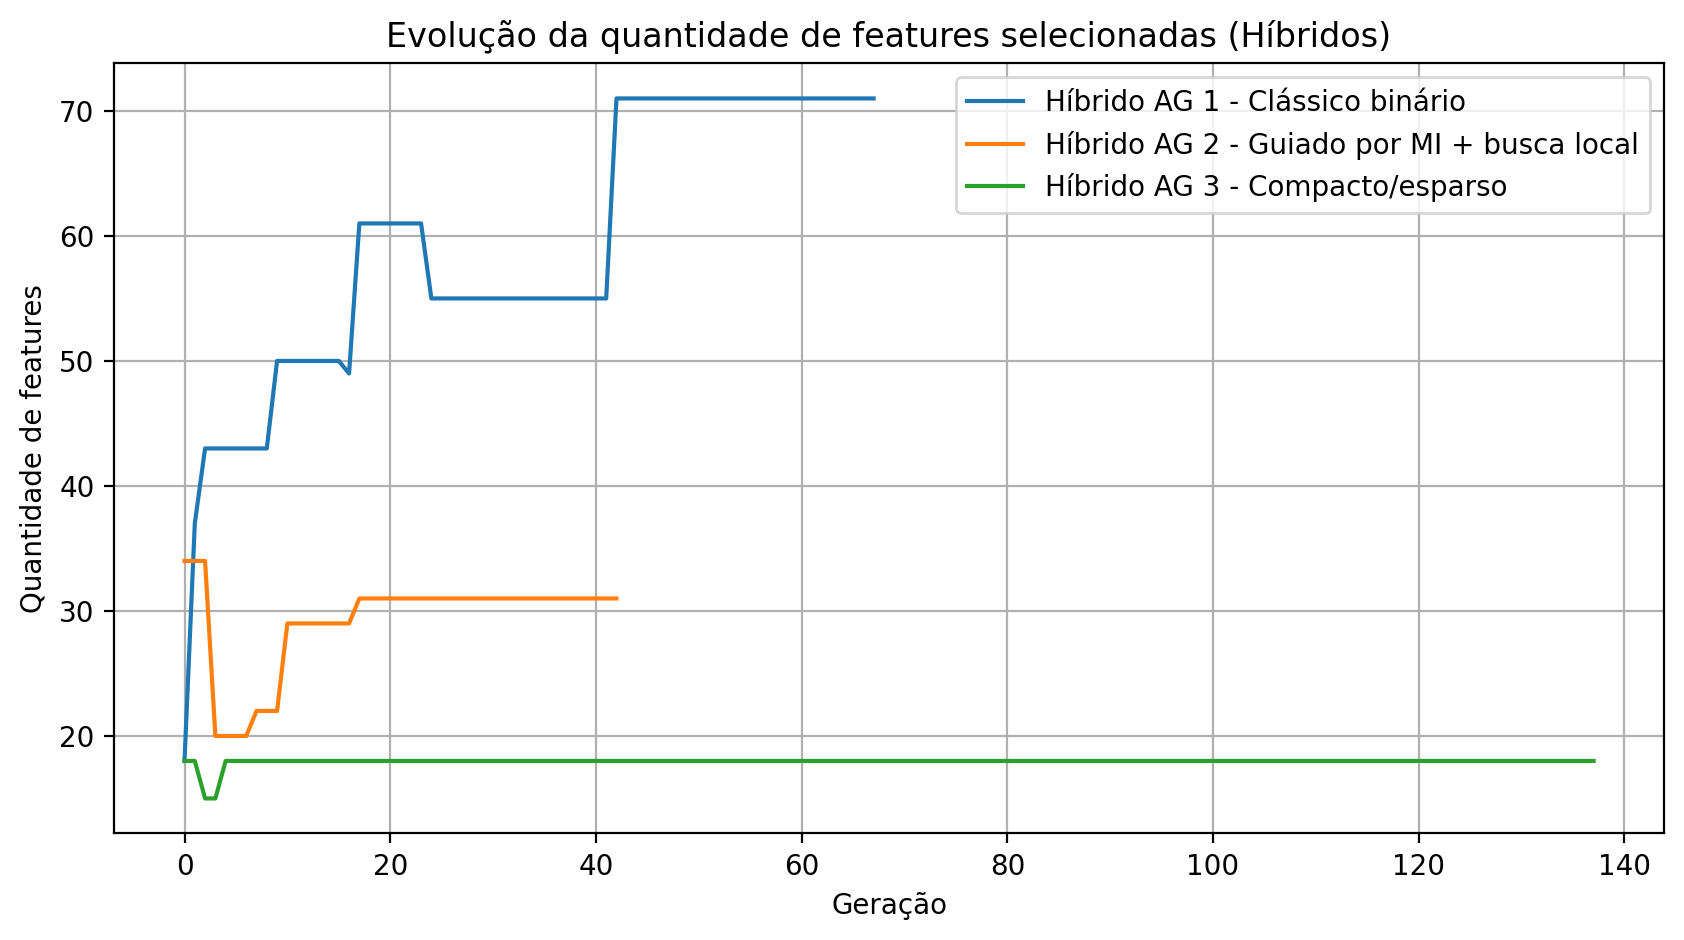
\includegraphics[width=.4\textwidth]{figures/evolution_ag_hybrid_n_features.png}
\end{figure}
\end{frame}

\begin{frame}{Resultados - Nível Base}

Os desempenhos individuais dos classificadores oscilam significativamente de acordo com cada dataset (reforçando o teorema "No Free Lunch").

\begin{figure}[H]
\centering
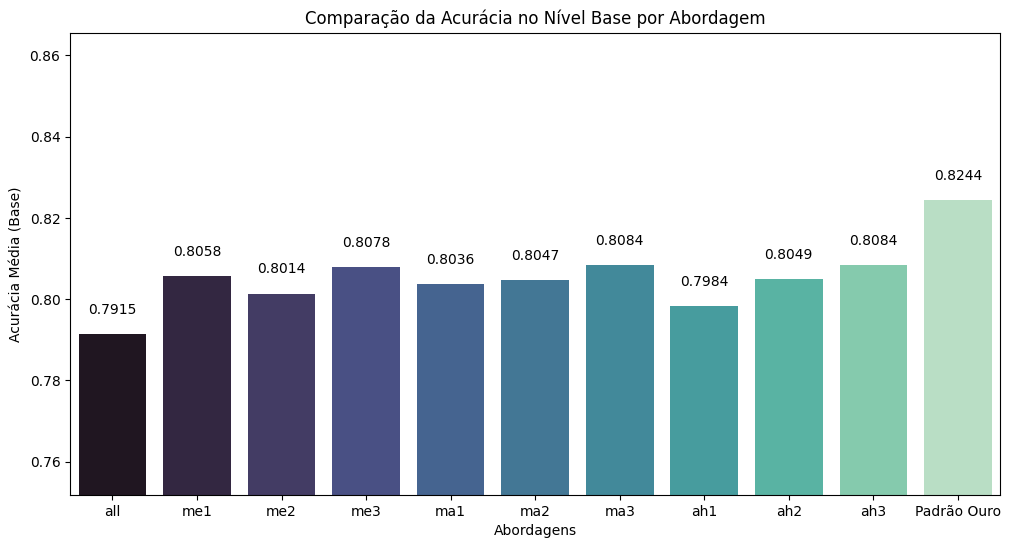
\includegraphics[width=.7\textwidth]{figures/acc_base.png}
\end{figure}
\end{frame}

\begin{frame}{Resultados - Nível Meta}

O emprego de Metamodelos para recomendação ativa alavanca e estabiliza os acertos globais do sistema.

\begin{figure}[H]
\centering
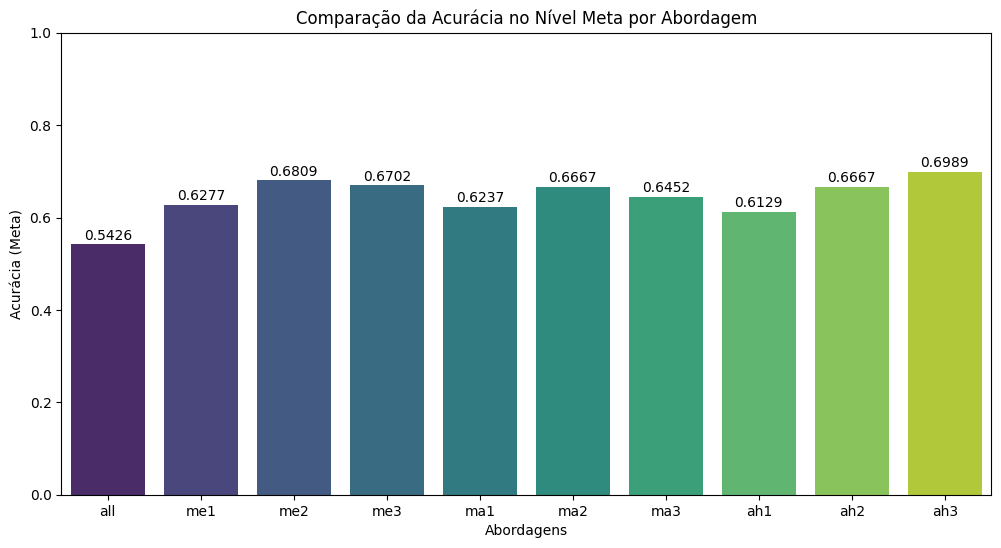
\includegraphics[width=.7\textwidth]{figures/acc_meta.png}
\end{figure}
\end{frame}

\section{Conclusão}

\begin{frame}{Conclusão}
\begin{block}{Principais Descobertas}
\begin{itemize}
    \item \textbf{Exatos:} Garantem podas rigorosas, mitigam redundância com chancela global (Mochila Quadrática baseada em correlação).
    \item \textbf{Aproximados:} Algoritmo guiado por MI obteve bom equilíbrio exploratório.
    \item \textbf{Híbridos:} Injeção da elite prematura gerou a \textbf{melhor solução preditiva (71\% com menos de 2\% dos dados brutos)}.
\end{itemize}
\end{block}

\vspace{0.3cm}
\begin{itemize}
    \item \textbf{Particularidade das meta-features:} As meta-features são descritivo, estatiticos e etc, por isso, os modelos baseados em árvores desempenhou melhor que os outros.
\end{itemize}
\begin{itemize}
    \item \textbf{Trade-off:} Modelos híbridos obtiveram a apoteose avaliativa em troca do alto fardo e custo de processamento sequencial. Alternativamente ao gargalo, estudos propõem abstrações transformando o espaço em contínuo \cite{metafs2023}.
\end{itemize}
\end{frame}

\section{Trabalhos Futuros}

\begin{frame}{Trabalhos Futuros}
\begin{block}{Perspectivas de Extensão}
Com base nos resultados e limitações deste estudo empírico, propõem-se as seguintes frentes para prosseguimento:
\end{block}

\vspace{0.3cm}
\begin{itemize}
    \item \textbf{Abordagem de Ranking:} Utilizar formulações baseadas em ordenação (\textit{ranking}) ao invés de classificação simples para a recomendação dos algoritmos.
    \item \textbf{Adoção de Múltiplas Métricas:} Expansão da avaliação sistêmica com a utilização de mais métricas de aprendizado de máquina, como F1-Score, Precisão e \textit{Recall}.
    \item \textbf{Benchmarking de Seleção:} Realizar \textit{benchmarking} comparativo estruturado com outros modelos e técnicas avançadas de seleção de meta-features disponíveis na literatura.
    \item \textbf{Diversificação da Base:} Verificar e validar a generalização dos métodos propostos em outros meta-datasets consolidados na literatura.
\end{itemize}
\end{frame}
\begin{frame}[allowframebreaks]{Referências}
    \bibliographystyle{plainnat}
    \bibliography{references}
\end{frame}

\begin{frame}{Agradecimentos}
    \centering
    {\color{uwopurple} \Huge \textbf{Obrigado}} 
\end{frame}

\end{document}